\documentclass[14pt]{extbook}
\usepackage{multicol, enumerate, enumitem, hyperref, color, soul, setspace, parskip, fancyhdr} %General Packages
\usepackage{amssymb, amsthm, amsmath, bbm, latexsym, units, mathtools} %Math Packages
\everymath{\displaystyle} %All math in Display Style
% Packages with additional options
\usepackage[headsep=0.5cm,headheight=12pt, left=1 in,right= 1 in,top= 1 in,bottom= 1 in]{geometry}
\usepackage[usenames,dvipsnames]{xcolor}
\usepackage{dashrule}  % Package to use the command below to create lines between items
\newcommand{\litem}[1]{\item#1\hspace*{-1cm}\rule{\textwidth}{0.4pt}}
\pagestyle{fancy}
\lhead{Progress Quiz 9}
\chead{}
\rhead{Version A}
\lfoot{8590-6105}
\cfoot{}
\rfoot{Fall 2020}
\begin{document}

\begin{enumerate}
\litem{
Solve the equation below. Then, choose the interval that contains the solution.\[ -19(7x + 15) = -9(-18x + 12) \]\begin{enumerate}[label=\Alph*.]
\item \( x \in [13.34, 13.68] \)
\item \( x \in [-1.27, -0.5] \)
\item \( x \in [1.27, 1.56] \)
\item \( x \in [-1.41, -1.14] \)
\item \( \text{There are no real solutions.} \)

\end{enumerate} }
\litem{
Solve the linear equation below. Then, choose the interval that contains the solution.\[ \frac{-9x + 8}{7} - \frac{-6x + 5}{4} = \frac{4x -7}{2} \]\begin{enumerate}[label=\Alph*.]
\item \( x \in [1.4, 2.3] \)
\item \( x \in [2.6, 3.8] \)
\item \( x \in [5.4, 6.1] \)
\item \( x \in [0.1, 1.6] \)
\item \( \text{There are no real solutions.} \)

\end{enumerate} }
\litem{
Solve the equation below. Then, choose the interval that contains the solution.\[ -3(14x -17) = -2(9x + 8) \]\begin{enumerate}[label=\Alph*.]
\item \( x \in [-2.3, -1.25] \)
\item \( x \in [-0.39, 0.8] \)
\item \( x \in [1.11, 1.92] \)
\item \( x \in [2.61, 2.83] \)
\item \( \text{There are no real solutions.} \)

\end{enumerate} }
\litem{
Write the equation of the line in the graph below in Standard form $Ax+By=C$. Then, choose the intervals that contain $A, B, \text{ and } C$.
\begin{center}
    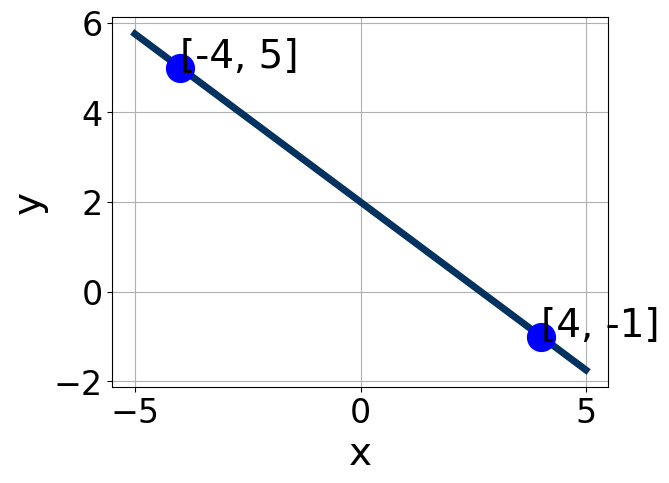
\includegraphics[width=0.5\textwidth]{../Figures/linearGraphToStandardCopyA.png}
\end{center}
\begin{enumerate}[label=\Alph*.]
\item \( A \in [1, 6], \hspace{3mm} B \in [-5.92, -3.55], \text{ and } \hspace{3mm} C \in [-4, 2] \)
\item \( A \in [-1.4, 0.6], \hspace{3mm} B \in [-1.42, -0.34], \text{ and } \hspace{3mm} C \in [-4, 2] \)
\item \( A \in [-1.4, 0.6], \hspace{3mm} B \in [0.32, 1.3], \text{ and } \hspace{3mm} C \in [-4, 2] \)
\item \( A \in [1, 6], \hspace{3mm} B \in [4.42, 5.49], \text{ and } \hspace{3mm} C \in [-4, 2] \)
\item \( A \in [-4, -1], \hspace{3mm} B \in [4.42, 5.49], \text{ and } \hspace{3mm} C \in [-4, 2] \)

\end{enumerate} }
\litem{
Solve the linear equation below. Then, choose the interval that contains the solution.\[ \frac{3x -3}{7} - \frac{-9x -6}{5} = \frac{6x -3}{4} \]\begin{enumerate}[label=\Alph*.]
\item \( x \in [-9, -7.6] \)
\item \( x \in [-1.4, 1.1] \)
\item \( x \in [-2.8, -1.3] \)
\item \( x \in [1, 1.4] \)
\item \( \text{There are no real solutions.} \)

\end{enumerate} }
\litem{
Find the equation of the line described below. Write the linear equation as $ y=mx+b $ and choose the intervals that contain $m$ and $b$.\[ \text{Perpendicular to } 8 x - 3 y = 8 \text{ and passing through the point } (4, -6). \]\begin{enumerate}[label=\Alph*.]
\item \( m \in [-3.2, -1.3] \hspace*{3mm} b \in [-6.2, -3.3] \)
\item \( m \in [0.2, 2.5] \hspace*{3mm} b \in [-7.6, -6.2] \)
\item \( m \in [-0.9, -0.2] \hspace*{3mm} b \in [-11.6, -8.7] \)
\item \( m \in [-0.9, -0.2] \hspace*{3mm} b \in [2.3, 6] \)
\item \( m \in [-0.9, -0.2] \hspace*{3mm} b \in [-6.2, -3.3] \)

\end{enumerate} }
\litem{
Find the equation of the line described below. Write the linear equation as $ y=mx+b $ and choose the intervals that contain $m$ and $b$.\[ \text{Perpendicular to } 8 x - 5 y = 4 \text{ and passing through the point } (2, 7). \]\begin{enumerate}[label=\Alph*.]
\item \( m \in [-3.76, -1.18] \hspace*{3mm} b \in [8.24, 8.42] \)
\item \( m \in [-0.77, -0.08] \hspace*{3mm} b \in [4.61, 5.39] \)
\item \( m \in [-0.77, -0.08] \hspace*{3mm} b \in [-8.35, -7.75] \)
\item \( m \in [0.01, 1.4] \hspace*{3mm} b \in [5.73, 5.85] \)
\item \( m \in [-0.77, -0.08] \hspace*{3mm} b \in [8.24, 8.42] \)

\end{enumerate} }
\litem{
Write the equation of the line in the graph below in Standard form $Ax+By=C$. Then, choose the intervals that contain $A, B, \text{ and } C$.
\begin{center}
    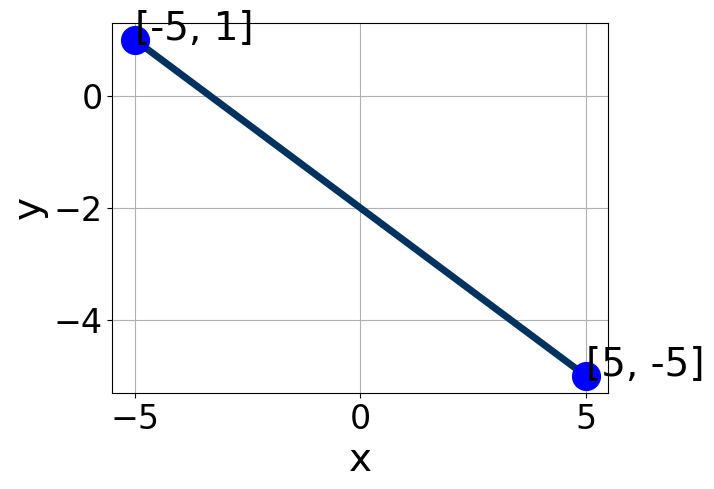
\includegraphics[width=0.5\textwidth]{../Figures/linearGraphToStandardA.png}
\end{center}
\begin{enumerate}[label=\Alph*.]
\item \( A \in [-0.75, 3.25], \hspace{3mm} B \in [-2, 0.3], \text{ and } \hspace{3mm} C \in [-7, -2] \)
\item \( A \in [3, 8], \hspace{3mm} B \in [3.5, 7.3], \text{ and } \hspace{3mm} C \in [18, 21] \)
\item \( A \in [3, 8], \hspace{3mm} B \in [-4.4, -1.5], \text{ and } \hspace{3mm} C \in [-26, -15] \)
\item \( A \in [-9, 1], \hspace{3mm} B \in [-4.4, -1.5], \text{ and } \hspace{3mm} C \in [-26, -15] \)
\item \( A \in [-0.75, 3.25], \hspace{3mm} B \in [-0.5, 2.9], \text{ and } \hspace{3mm} C \in [0, 7] \)

\end{enumerate} }
\litem{
First, find the equation of the line containing the two points below. Then, write the equation as $ y=mx+b $ and choose the intervals that contain $m$ and $b$.\[ (7, -2) \text{ and } (-8, 3) \]\begin{enumerate}[label=\Alph*.]
\item \( m \in [-0.87, 0.22] \hspace*{3mm} b \in [10.72, 11.39] \)
\item \( m \in [-0.87, 0.22] \hspace*{3mm} b \in [-0.14, 0.73] \)
\item \( m \in [-0.87, 0.22] \hspace*{3mm} b \in [-1, 0.27] \)
\item \( m \in [-0.01, 1.14] \hspace*{3mm} b \in [5.32, 6.4] \)
\item \( m \in [-0.87, 0.22] \hspace*{3mm} b \in [-9.53, -8.79] \)

\end{enumerate} }
\litem{
First, find the equation of the line containing the two points below. Then, write the equation as $ y=mx+b $ and choose the intervals that contain $m$ and $b$.\[ (-7, 10) \text{ and } (10, -7) \]\begin{enumerate}[label=\Alph*.]
\item \( m \in [-4, 0] \hspace*{3mm} b \in [-1, 12] \)
\item \( m \in [0, 4] \hspace*{3mm} b \in [-19, -14] \)
\item \( m \in [-4, 0] \hspace*{3mm} b \in [-19, -14] \)
\item \( m \in [-4, 0] \hspace*{3mm} b \in [15, 24] \)
\item \( m \in [-4, 0] \hspace*{3mm} b \in [-7, -2] \)

\end{enumerate} }
\end{enumerate}

\end{document}